%%%%%%%%%%%%%%%%%%%%%%%%%%%%%%%%%%%%%%%%%%%%%%%%%%%%%%%%%%%%%%%%%%%%%%%%%
% Template for a revtex article
%%%%%%%%%%%%%%%%%%%%%%%%%%%%%%%%%%%%%%%%%%%%%%%%%%%%%%%%%%%%%%%%%%%%%%%%%
\documentclass[rmp]{revtex4}
%%%%%%%%%%%%%%%%%%%%%%%%%%%%%%%%%%%%%%%%%%%%%%%%%%%%%%%%%%%%%%%%%%%%%%%%%
\usepackage[english]{babel}
\usepackage[utf8x]{inputenc}
\usepackage{amsmath,amsfonts,amssymb,eucal,eurosym,textcomp}
\usepackage{color}
\usepackage{graphicx}
\usepackage[caption=false]{subfig}
\usepackage{natbib}
\usepackage{pslatex}
\usepackage[colorlinks,linkcolor=red,citecolor=red]{hyperref}
%%%%%%%%%%%%%%%%%%%%%%%%%%%%%%%%%%%%%%%%%%%%%%%%%%%%%%%%%%%%%%%%%%%%%%%%%
\graphicspath{{./figures/}}
%%%%%%%%%%%%%%%%%%%%%%%%%%%%%%%%%%%%%%%%%%%%%%%%%%%%%%%%%%%%%%%%%%%%%%%%%
\newcommand{\comment}[1]{{\color{red}#1}}
%%%%%%%%%%%%%%%%%%%%%%%%%%%%%%%%%%%%%%%%%%%%%%%%%%%%%%%%%%%%%%%%%%%%%%%%%
\renewcommand{\thesubfigure}{\Alph{subfigure}}
\newcommand{\Author}{Fabio~Zanini* and Richard~A.~Neher*}
\newcommand{\Title}{Deleterious synonymous mutations hitchhike to high frequency in HIV \env~evolution}
\newcommand{\Affiliation}{Max Planck Institute for Developmental Biology, 72076 T\"ubingen, Germany}
%\hypersetup{pdfauthor={\Author}, pdftitle={\Title}, pdfkeywords={\Keywords}}
%%%%%%%%%%%%%%%%%%%%%%%%%%%%%%%%%%%%%%%%%%%%%%%%%%%%%%%%%%%%%%%%%%%%%%%%%
\begin{document}
%%%%%%%%%%%%%%%%%%%%%%%%%%%%%%%%%%%%%%%%%%%%%%%%%%%%%%%%%%%%%%%%%%%%%%%%%
\title{\Title}
\author{\Author}
\affiliation{\textsf{*}\Affiliation}
\date{\today}
\maketitle
%%%%%%%%%%%%%%%%%%%%%%%%%%%%%%%%%%%%%%%%%%%%%%%%%%%%%%%%%%%%%%%%%%%%%%%%%
\tableofcontents

%%%%%%%%%%%%%%%%%%%%%%%%%%%%%%%%%%%%%%%%%%%%%%%%%%%%%%%%%%%%%%%%%%%%%%%%%
\section{Selection of the patient data}
%%%%%%%%%%%%%%%%%%%%%%%%%%%%%%%%%%%%%%%%%%%%%%%%%%%%%%%%%%%%%%%%%%%%%%%%%
\begin{figure}[ht]
\begin{center}
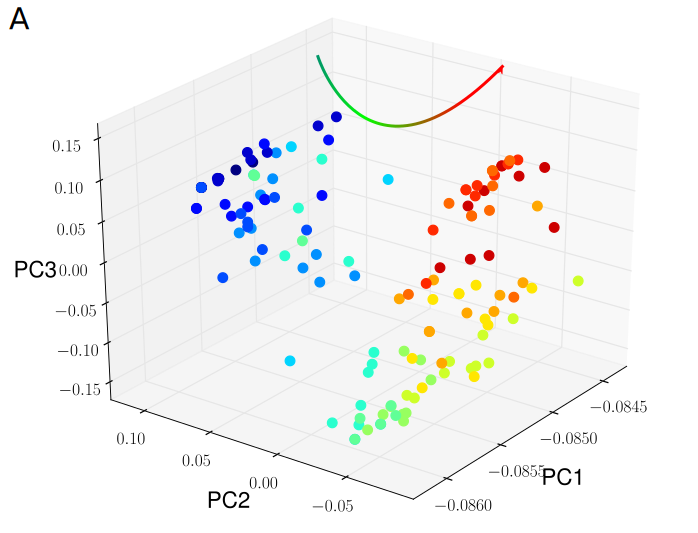
\includegraphics[width=0.4\linewidth]{Shankarappa_PCA_p1}
\includegraphics[width=0.4\linewidth]{Shankarappa_allele_freqs_trajectories_nonsyn_p1}
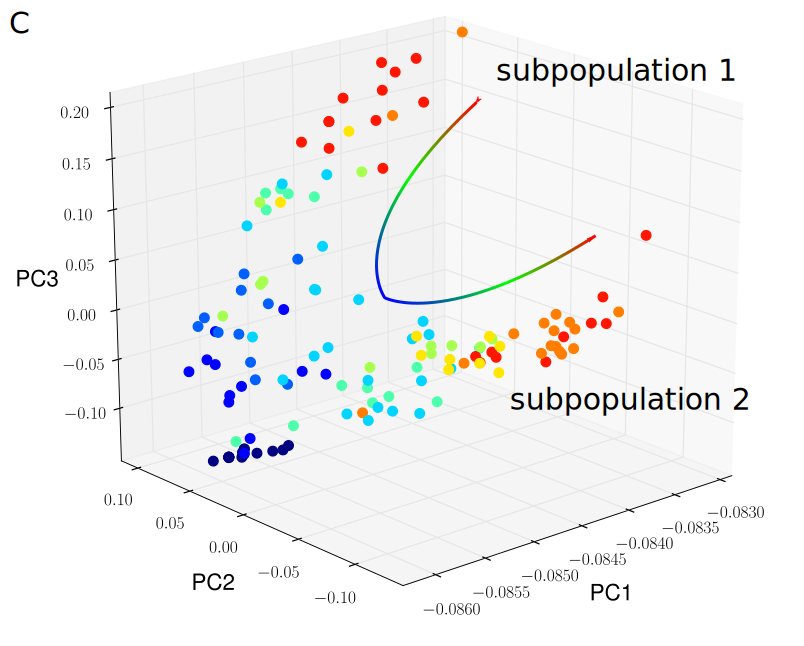
\includegraphics[width=0.4\linewidth]{Shankarappa_PCA_p7}
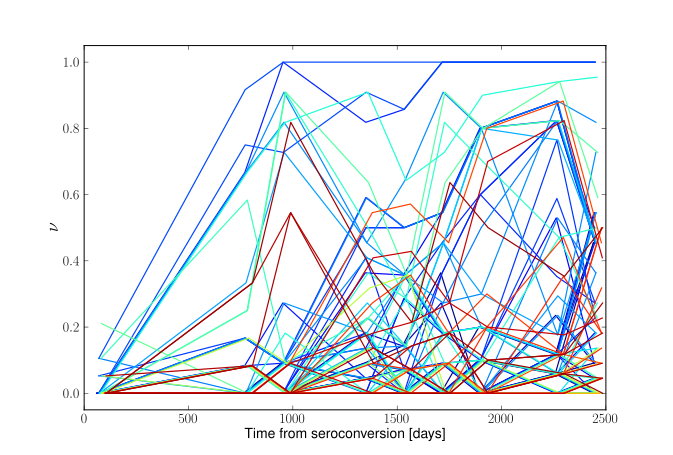
\includegraphics[width=0.4\linewidth]{Shankarappa_allele_freqs_trajectories_nonsyn_p7}
\caption{Panel A) PCA of all sequences from patient p1 (colors indicate time from seroconversion,
from blue to red). Panel B) Allele frequency trajectories for nonsynonymous
changes in the same patient. Panels C and D) show analogous plots for data from
patient p7. Samples after day 1000 split into two clusters in the PCA and no
mutations that arise after day 1000 fix, presumably because they are restricted
to one subpopulation. }
\label{fig:aftp}
\end{center}
\end{figure}
Patients p4, p7, p8, p9 from ref.~\citealp{shankarappa_consistent_1999} and
patients ACH19542 and ACH19768 from ref.~\citealp{bunnik_autologous_2008} showed clear signs of
compartimentalization (population structure) during infection. This population
structure is easy to spot after a principle component analysis (PCA) of all
sequences from all samples from one patients. When the projections onto the
first 3 PCs for each sequence, the above mentioned patients show bifurcation
into two clusters at later time points. Since mutations that arise in one subpopulation cannot fix population wide, such population
structure confounds our analysis and these patients were exclude.


Similar, but less obvious, conclusions can be drawn from the allele frequency
trajectories plotted next to the PCA plots: no allele that arose after 1000
days from seroconversion ever fixes, but a most mutations hover at frequencies
around 0.5-0.8. Fluctuations of these allele frequencies probably reflect
changing relative sizes of the subpopulations. 

%%%%%%%%%%%%%%%%%%%%%%%%%%%%%%%%%%%%%%%%%%%%%%%%%%%%%%%%%%%%%%%%%%%%%%%%%
\section{Nonsynonymous changes outside of variable regions are deleterious}
%%%%%%%%%%%%%%%%%%%%%%%%%%%%%%%%%%%%%%%%%%%%%%%%%%%%%%%%%%%%%%%%%%%%%%%%%
\begin{figure}[h]
\begin{center}
\includegraphics[width=0.5\linewidth]{synmut_conservation_4fold_synnonsyn}
\caption{Cumulative distribution of synonymous and nonsynonymous diversity in
{\it gag} in the LANL reference panel. Nonsynonymous sites are much
less diverse than 4-fold synonymous sites. \comment{The title is wrong. How
do you decide on 4-fold degeneracy? (consensus amino acid???)}.}
\label{fig:synnonsyncons}
\end{center}
\end{figure}
\comment{this can use streamlining. Why not put is all into the figure caption}
In the main text, it is argued that, whereas the deleterious effect of
synonymous changes is very small, most nonsynonymous mutations outside of the
variable regions are much worse. To show this, we take a multiple sequence alignment of
the {\it gag} gene of subtype-B HIV sequences from the LANL website (filtered
sequences only, version 2011)~\cite{LANL2012} and look at diversity at fourfold degenerate
codons. The ratio of observed versus possible mutations is much lower for
nonsynonymous changes than synonymous ones, as shown in
\figurename~\ref{fig:synnonsyncons} in a cumulative histogram. From this
evidence (which is highly statistically significant) we conclude that, as a
general rule, nonsynonymous changes that are not currently escape mutations
are likely to incur in large fitness costs.

%%%%%%%%%%%%%%%%%%%%%%%%%%%%%%%%%%%%%%%%%%%%%%%%%%%%%%%%%%%%%%%%%%%%%%%%%
\section{Synonymous diversity across the HIV genome}
%%%%%%%%%%%%%%%%%%%%%%%%%%%%%%%%%%%%%%%%%%%%%%%%%%%%%%%%%%%%%%%%%%%%%%%%%
\begin{figure}[h]
\begin{center}
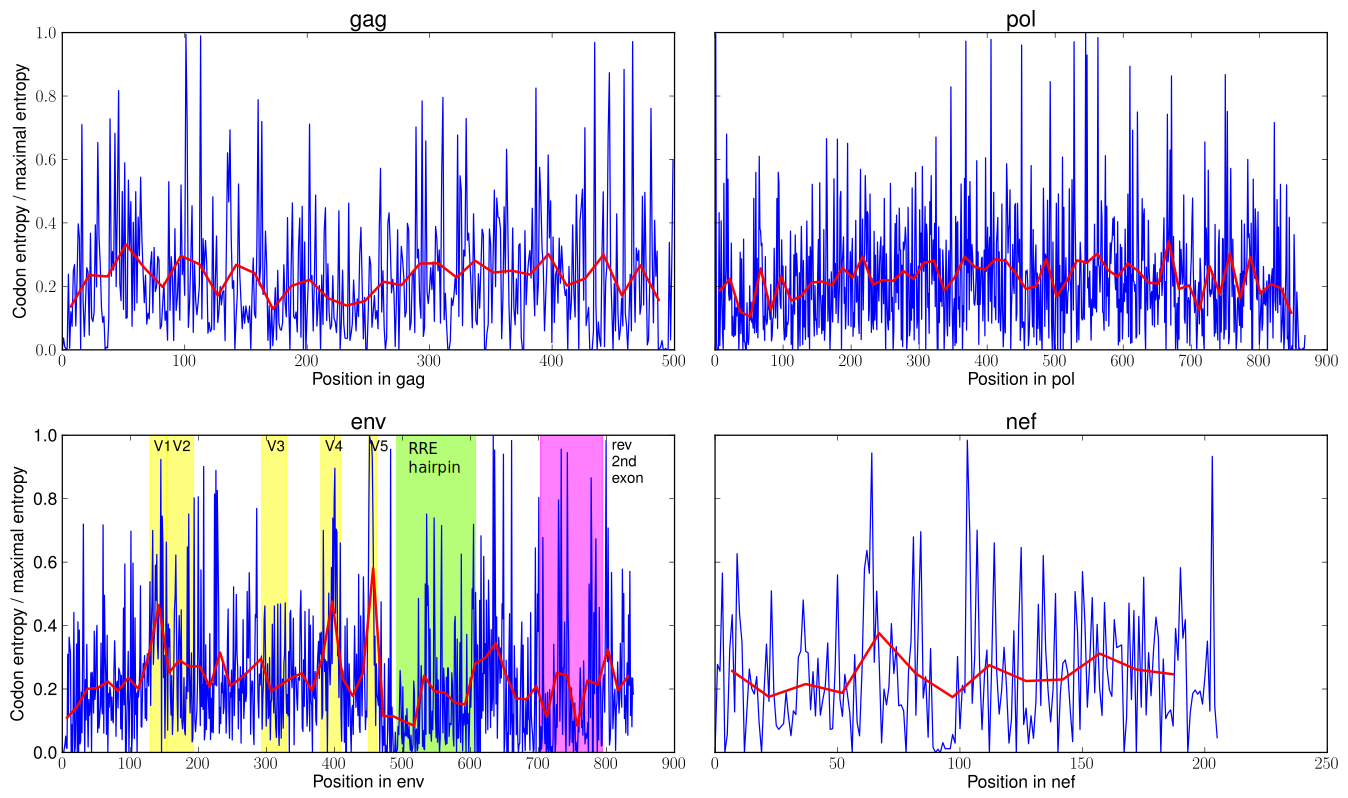
\includegraphics[width=\linewidth]{conservation_codons_genome}
\caption{Normalized codon entropy across the HIV genome is clustered around
variable regions in {\it env}.}
\label{fig:syndiv_genome}
\end{center}
\end{figure}

Our analysis relies on the ability of synonymous mutation to reach high
frequencies within the viral population (by hitchhiking). The ability of HIV to
explore the synonymous mutational space can be quantified by the codon entropy.
Using a multiple sequence alignment of subtype-B HIV sequences from the LANL
website (filtered sequences only, version 2011)~\cite{LANL2012}, we show in
\figurename~\ref{fig:syndiv_genome} that the genomic regions within and flanking
V loops contain the highest codon entropy (normalized by the maximal entropy for
each degenerate codon). On the contrary, regions that are under selection either
the the RNA level (the RRE hairpin) or at the protein level but in a different
reading frame (rev second exon), show reduced entropy, i.e. more constrains.

All parts of {\it env} that are part of a different gene have been excluded from
our main analysis, to avoid contamination about synonymity.

%%%%%%%%%%%%%%%%%%%%%%%%%%%%%%%%%%%%%%%%%%%%%%%%%%%%%%%%%%%%%%%%%%%%%%%%%
\section{Alternative models for suppression of nonsynonymous mutations}
%%%%%%%%%%%%%%%%%%%%%%%%%%%%%%%%%%%%%%%%%%%%%%%%%%%%%%%%%%%%%%%%%%%%%%%%%
\begin{figure}[h]
\begin{center}
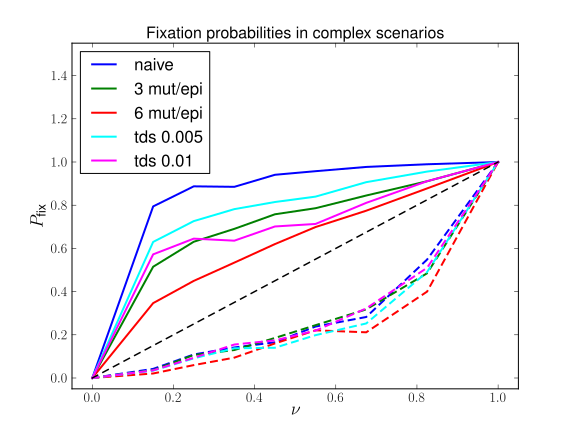
\includegraphics[width=0.5\linewidth]{simulations_graduallyepitopesandtimeselec}
\caption{Time-dependent selection (the escape mutant is recognized after some
months from its appearance) and competition between escape mutations in the same
epitope both reduce fixation of nonsynonymous mutations, without affecting the
synonymous curve much.}
\label{fig:tds_wec}
\end{center}
\end{figure}
As mentioned in the main text, both competition of different mutants within the
same allele and a slow, catching-up immune system can reduce the fixation
probability of nonsynonymous derived alleles. This is observed in computer
models, an example of which is shown in \figurename~\ref{fig:tds_wec}. In the
curves denoted with ``tds'' (time-dependent selection), the fitness advantage of
an escape mutaition can vanish at each time point with a probability density
\[ P_\text{recognized}(t) = c \cdot \nu(t), \]
where $c$ is a constant coefficient shown in the legend that encodes the overall
efficiency of the host immune system, and $\nu(t)$ is the frequency of the
escape allele at time $t$. The curves denoted with ``mut/epi'' describe the
competition scenario instead, with 3 or 6 escape mutations within the same
epitope of length 9 nucleotides. Increasing either the coefficient $c$ or the
number of escape mutants per epitope reduces fixation of nonsynonymous derived
alleles. Importantly, the synonymous fixation probability is hardly affected, which casts
trust over the main conclusions of the main text independently on the details of
the selection scenario at the protein level.

%%%%%%%%%%%%%%%%%%%%%%%%%%%%%%%%%%%%%%%%%%%%%%%%%%%%%%%%%%%%%%%%%%%%%%%%%
\bibliographystyle{natbib}
\bibliography{bib}
%%%%%%%%%%%%%%%%%%%%%%%%%%%%%%%%%%%%%%%%%%%%%%%%%%%%%%%%%%%%%%%%%%%%%%%%%
\end{document}
%%%%%%%%%%%%%%%%%%%%%%%%%%%%%%%%%%%%%%%%%%%%%%%%%%%%%%%%%%%%%%%%%%%%%%%%%

